\section{Evaluation protocol}
The primary comparison evaluates the wide MLP versus the depth-2 entangled QNN across all five benchmark datasets. Secondary experiments compare QNN depths 1, 2, and 3, compare depth 2 with versus without CNOT, and contrast the QNN against parameter-matched compact MLPs ($d\to2\to1$: 9 parameters on 2D datasets, 13 parameters on 4D datasets). Metrics are accuracy, precision, recall, F1-score, ROC AUC, binary log loss, and measured training time. Scores are reported as mean and sample standard deviation across paired runs.

For model comparisons, paired differences are calculated seed by seed:
\begin{equation}
  \Delta_i = \text{Metric}_{\text{QNN}, i} - \text{Metric}_{\text{Classical}, i}.
\end{equation}
A paired $t$-test and Wilcoxon signed-rank test are calculated alongside a 95\% confidence interval for the mean paired difference.

\subsection{Runtime and implementation details}
The same full-batch training schedule is used for all models: binary cross-entropy with logits, Adam optimizer, 100 epochs, no mini-batch sampling, weight decay $10^{-4}$, and gradient clipping at norm 5. The MLP learning rate is 0.01 and the QNN learning rate is 0.025.

Elapsed training time is measured strictly around the model training call on a single CPU thread. The primary PennyLane backend executes a batched Torch-interface QNode on \texttt{default.qubit} with analytic expectation values (\texttt{shots=None}). The reference backend uses explicit PyTorch tensor statevectors. QNode dispatch overhead materially affects absolute timing, which is why measured PennyLane execution times are explicitly reported.

\subsection{Finite-shot evaluation}
To inspect measurement sampling variability, the trained depth-2 QNN is evaluated using exact expectations and simulated multinomial measurements with 256 and 1,024 shots across five independent resamplings per split. Model weights are not retrained under finite-shot noise; this isolates inference shot sensitivity from optimization noise.

\section{Results}
\subsection{Primary QNN--MLP comparison across benchmarks}

\begin{table}[!htbp]
\centering\small
\caption{Primary test performance and training time (mean $\pm$ sample SD across paired runs).}
\begin{tabular}{@{}llrrrr@{}}
\toprule
Dataset & Model & Accuracy & F1-score & ROC AUC & Train time (s)\\
\midrule
PennyLane TFIM & Compact MLP (13p) & \pennylaneTfimMLPSmallAccuracy & \pennylaneTfimMLPSmallFOne & \pennylaneTfimMLPSmallRocAuc & \pennylaneTfimMLPSmallTrainTimeS\\
PennyLane TFIM & Wide MLP (225p) & \pennylaneTfimMLPAccuracy & \pennylaneTfimMLPFOne & \pennylaneTfimMLPRocAuc & \pennylaneTfimMLPTrainTimeS\\
PennyLane TFIM & QNN, depth 2 (13p) & \pennylaneTfimQNNdTwoEntAccuracy & \pennylaneTfimQNNdTwoEntFOne & \pennylaneTfimQNNdTwoEntRocAuc & \pennylaneTfimQNNdTwoEntTrainTimeS\\
\midrule
Qiskit Phase of Matter & Compact MLP (13p) & \qiskitPhaseOfMatterMLPSmallAccuracy & \qiskitPhaseOfMatterMLPSmallFOne & \qiskitPhaseOfMatterMLPSmallRocAuc & \qiskitPhaseOfMatterMLPSmallTrainTimeS\\
Qiskit Phase of Matter & Wide MLP (225p) & \qiskitPhaseOfMatterMLPAccuracy & \qiskitPhaseOfMatterMLPFOne & \qiskitPhaseOfMatterMLPRocAuc & \qiskitPhaseOfMatterMLPTrainTimeS\\
Qiskit Phase of Matter & QNN, depth 2 (13p) & \qiskitPhaseOfMatterQNNdTwoEntAccuracy & \qiskitPhaseOfMatterQNNdTwoEntFOne & \qiskitPhaseOfMatterQNNdTwoEntRocAuc & \qiskitPhaseOfMatterQNNdTwoEntTrainTimeS\\
\midrule
Havl\'i\v{c}ek Ad-Hoc & Compact MLP (9p) & \havlicekAdhocMLPSmallAccuracy & \havlicekAdhocMLPSmallFOne & \havlicekAdhocMLPSmallRocAuc & \havlicekAdhocMLPSmallTrainTimeS\\
Havl\'i\v{c}ek Ad-Hoc & Wide MLP (193p) & \havlicekAdhocMLPAccuracy & \havlicekAdhocMLPFOne & \havlicekAdhocMLPRocAuc & \havlicekAdhocMLPTrainTimeS\\
Havl\'i\v{c}ek Ad-Hoc & QNN, depth 2 (7p) & \havlicekAdhocQNNdTwoEntAccuracy & \havlicekAdhocQNNdTwoEntFOne & \havlicekAdhocQNNdTwoEntRocAuc & \havlicekAdhocQNNdTwoEntTrainTimeS\\
\midrule
Breast Cancer & Compact MLP (13p) & \breastCancerMLPSmallAccuracy & \breastCancerMLPSmallFOne & \breastCancerMLPSmallRocAuc & \breastCancerMLPSmallTrainTimeS\\
Breast Cancer & Wide MLP (225p) & \breastCancerMLPAccuracy & \breastCancerMLPFOne & \breastCancerMLPRocAuc & \breastCancerMLPTrainTimeS\\
Breast Cancer & QNN, depth 2 (13p) & \breastCancerQNNdTwoEntAccuracy & \breastCancerQNNdTwoEntFOne & \breastCancerQNNdTwoEntRocAuc & \breastCancerQNNdTwoEntTrainTimeS\\
\midrule
MNIST Digits (0 vs 1) & Compact MLP (13p) & \mnistDigitsMLPSmallAccuracy & \mnistDigitsMLPSmallFOne & \mnistDigitsMLPSmallRocAuc & \mnistDigitsMLPSmallTrainTimeS\\
MNIST Digits (0 vs 1) & Wide MLP (225p) & \mnistDigitsMLPAccuracy & \mnistDigitsMLPFOne & \mnistDigitsMLPRocAuc & \mnistDigitsMLPTrainTimeS\\
MNIST Digits (0 vs 1) & QNN, depth 2 (13p) & \mnistDigitsQNNdTwoEntAccuracy & \mnistDigitsQNNdTwoEntFOne & \mnistDigitsQNNdTwoEntRocAuc & \mnistDigitsQNNdTwoEntTrainTimeS\\
\bottomrule
\end{tabular}
\label{tab:primary}
\end{table}
\noindent\emph{Provenance note:} all metrics in Table~\ref{tab:primary} are injected directly from the automated PennyLane \texttt{default.qubit} pipeline run via LaTeX macros.

\begin{figure}[!htbp]
\centering
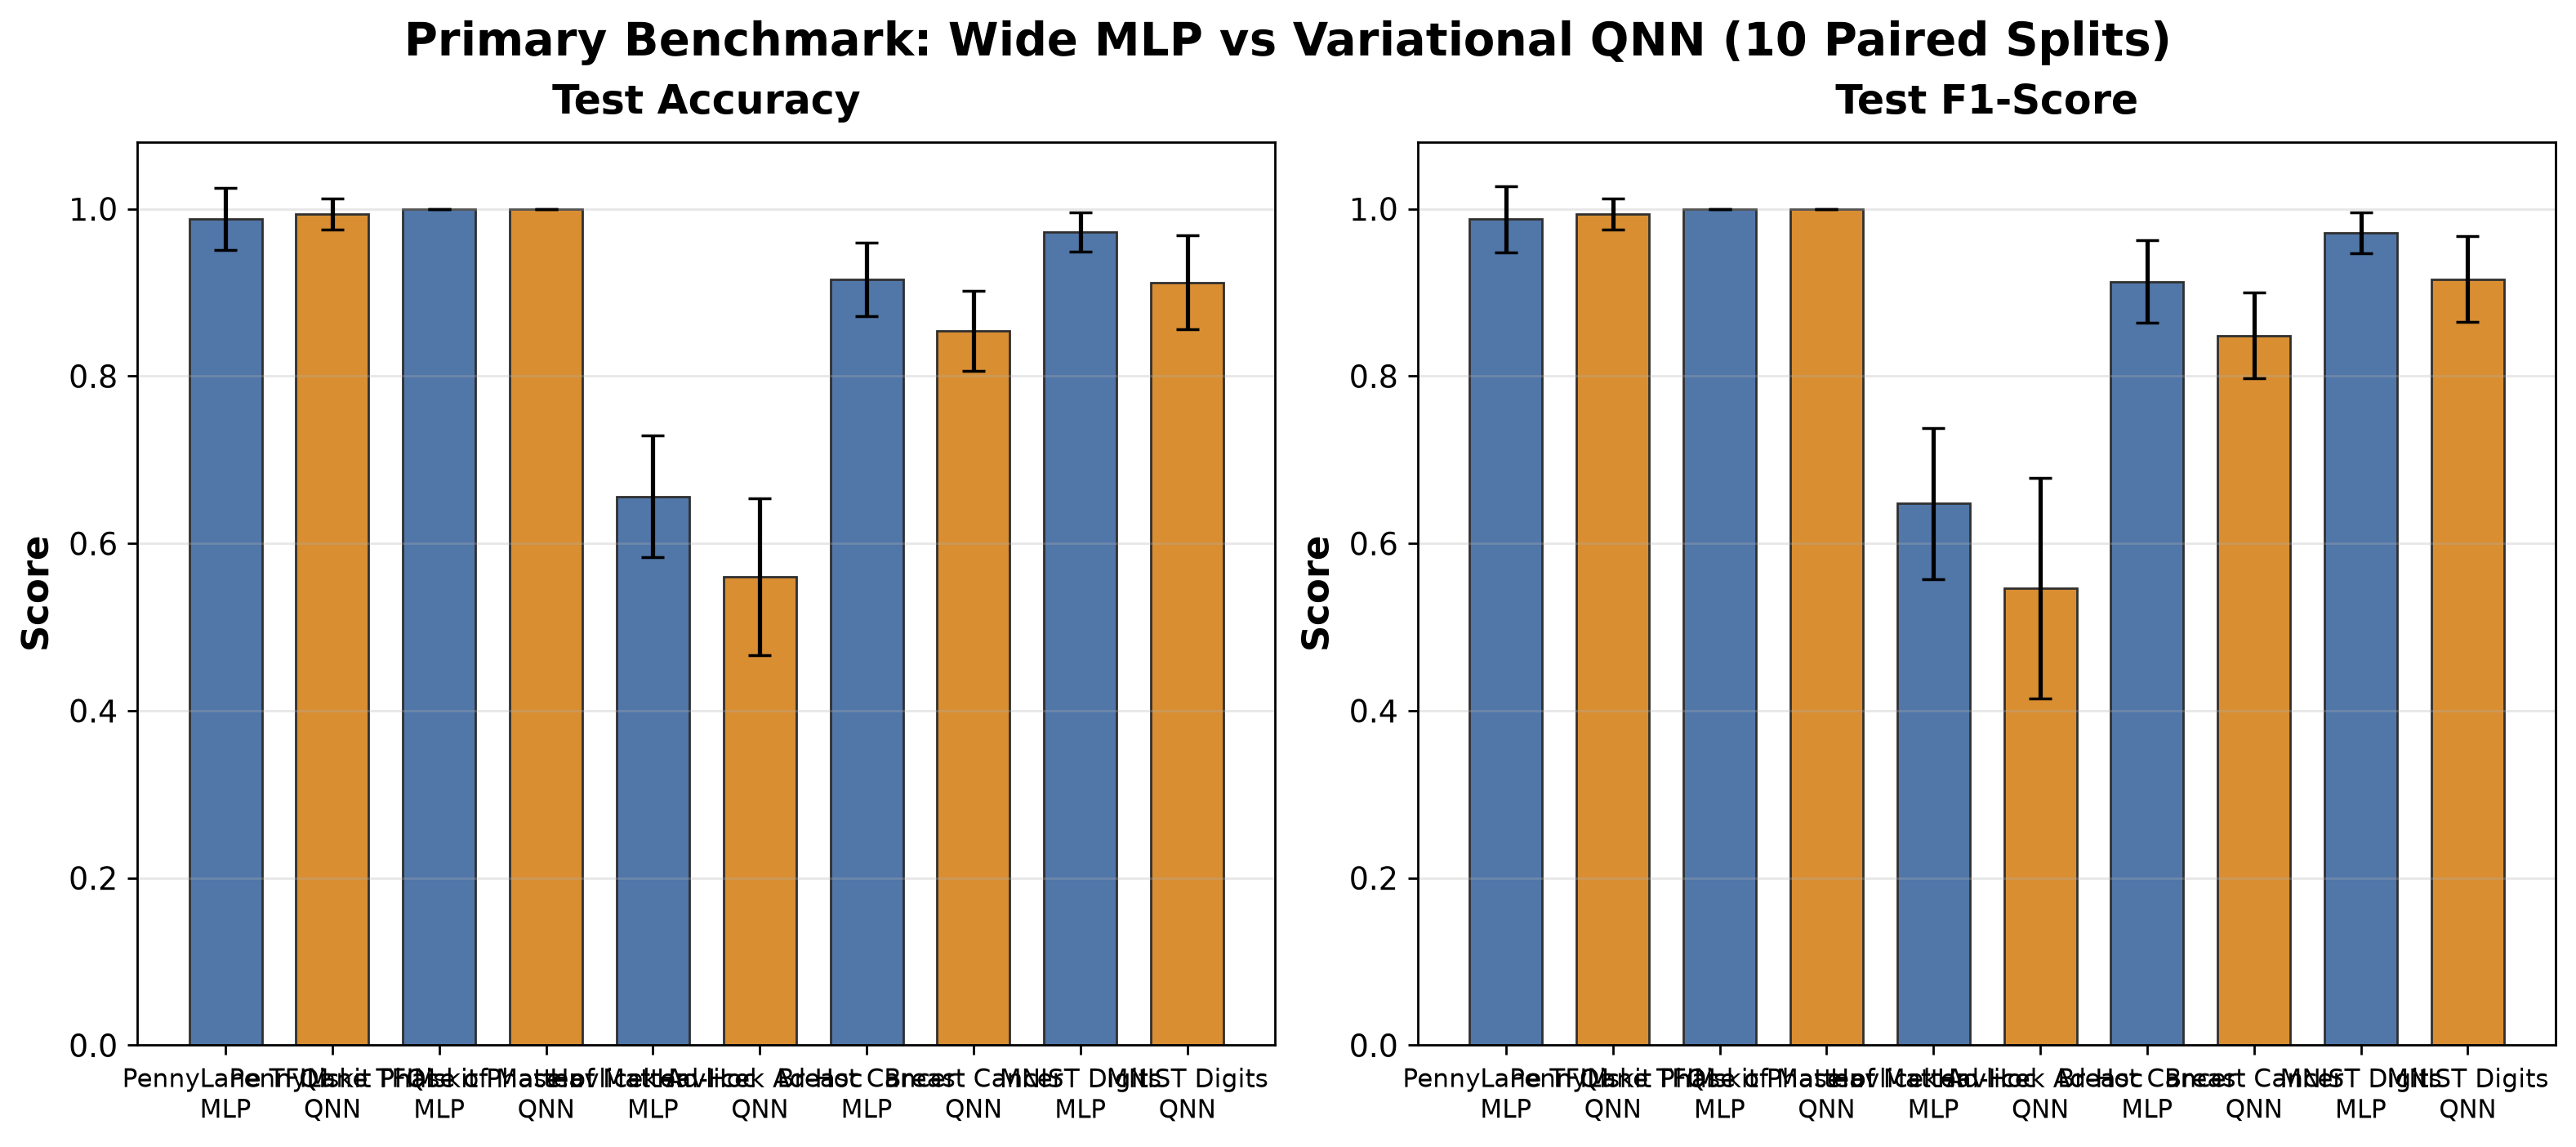
\includegraphics[width=0.98\linewidth]{results/figures/primary_metrics.png}
\caption{Accuracy and F1-score across all five benchmark distributions for the wide MLP and depth-2 QNN. Error bars show sample standard deviation across runs.}
\label{fig:primarymetrics}
\end{figure}

\subsection{Decision boundaries and learning curves}
Figure~\ref{fig:boundaries} displays the learned boundaries for all benchmark tasks on the seed-0 partition. On quantum state benchmarks (PennyLane TFIM and Qiskit Phase of Matter), both classical and quantum architectures successfully reconstruct the transition manifold separating distinct quantum phases from observable expectation features. On high-dimensional quantum kernel data (Havl\'i\v{c}ek benchmark), the non-linear decision boundary illustrates the interaction between data-reuploading layers and quantum feature maps, while classical MLPs form linear piecewise partitions. On classical small-data benchmarks (Breast Cancer and MNIST digits), both architectures isolate the diagnostic and morphological clusters with smooth decision margins.

\begin{figure}[p]
\centering
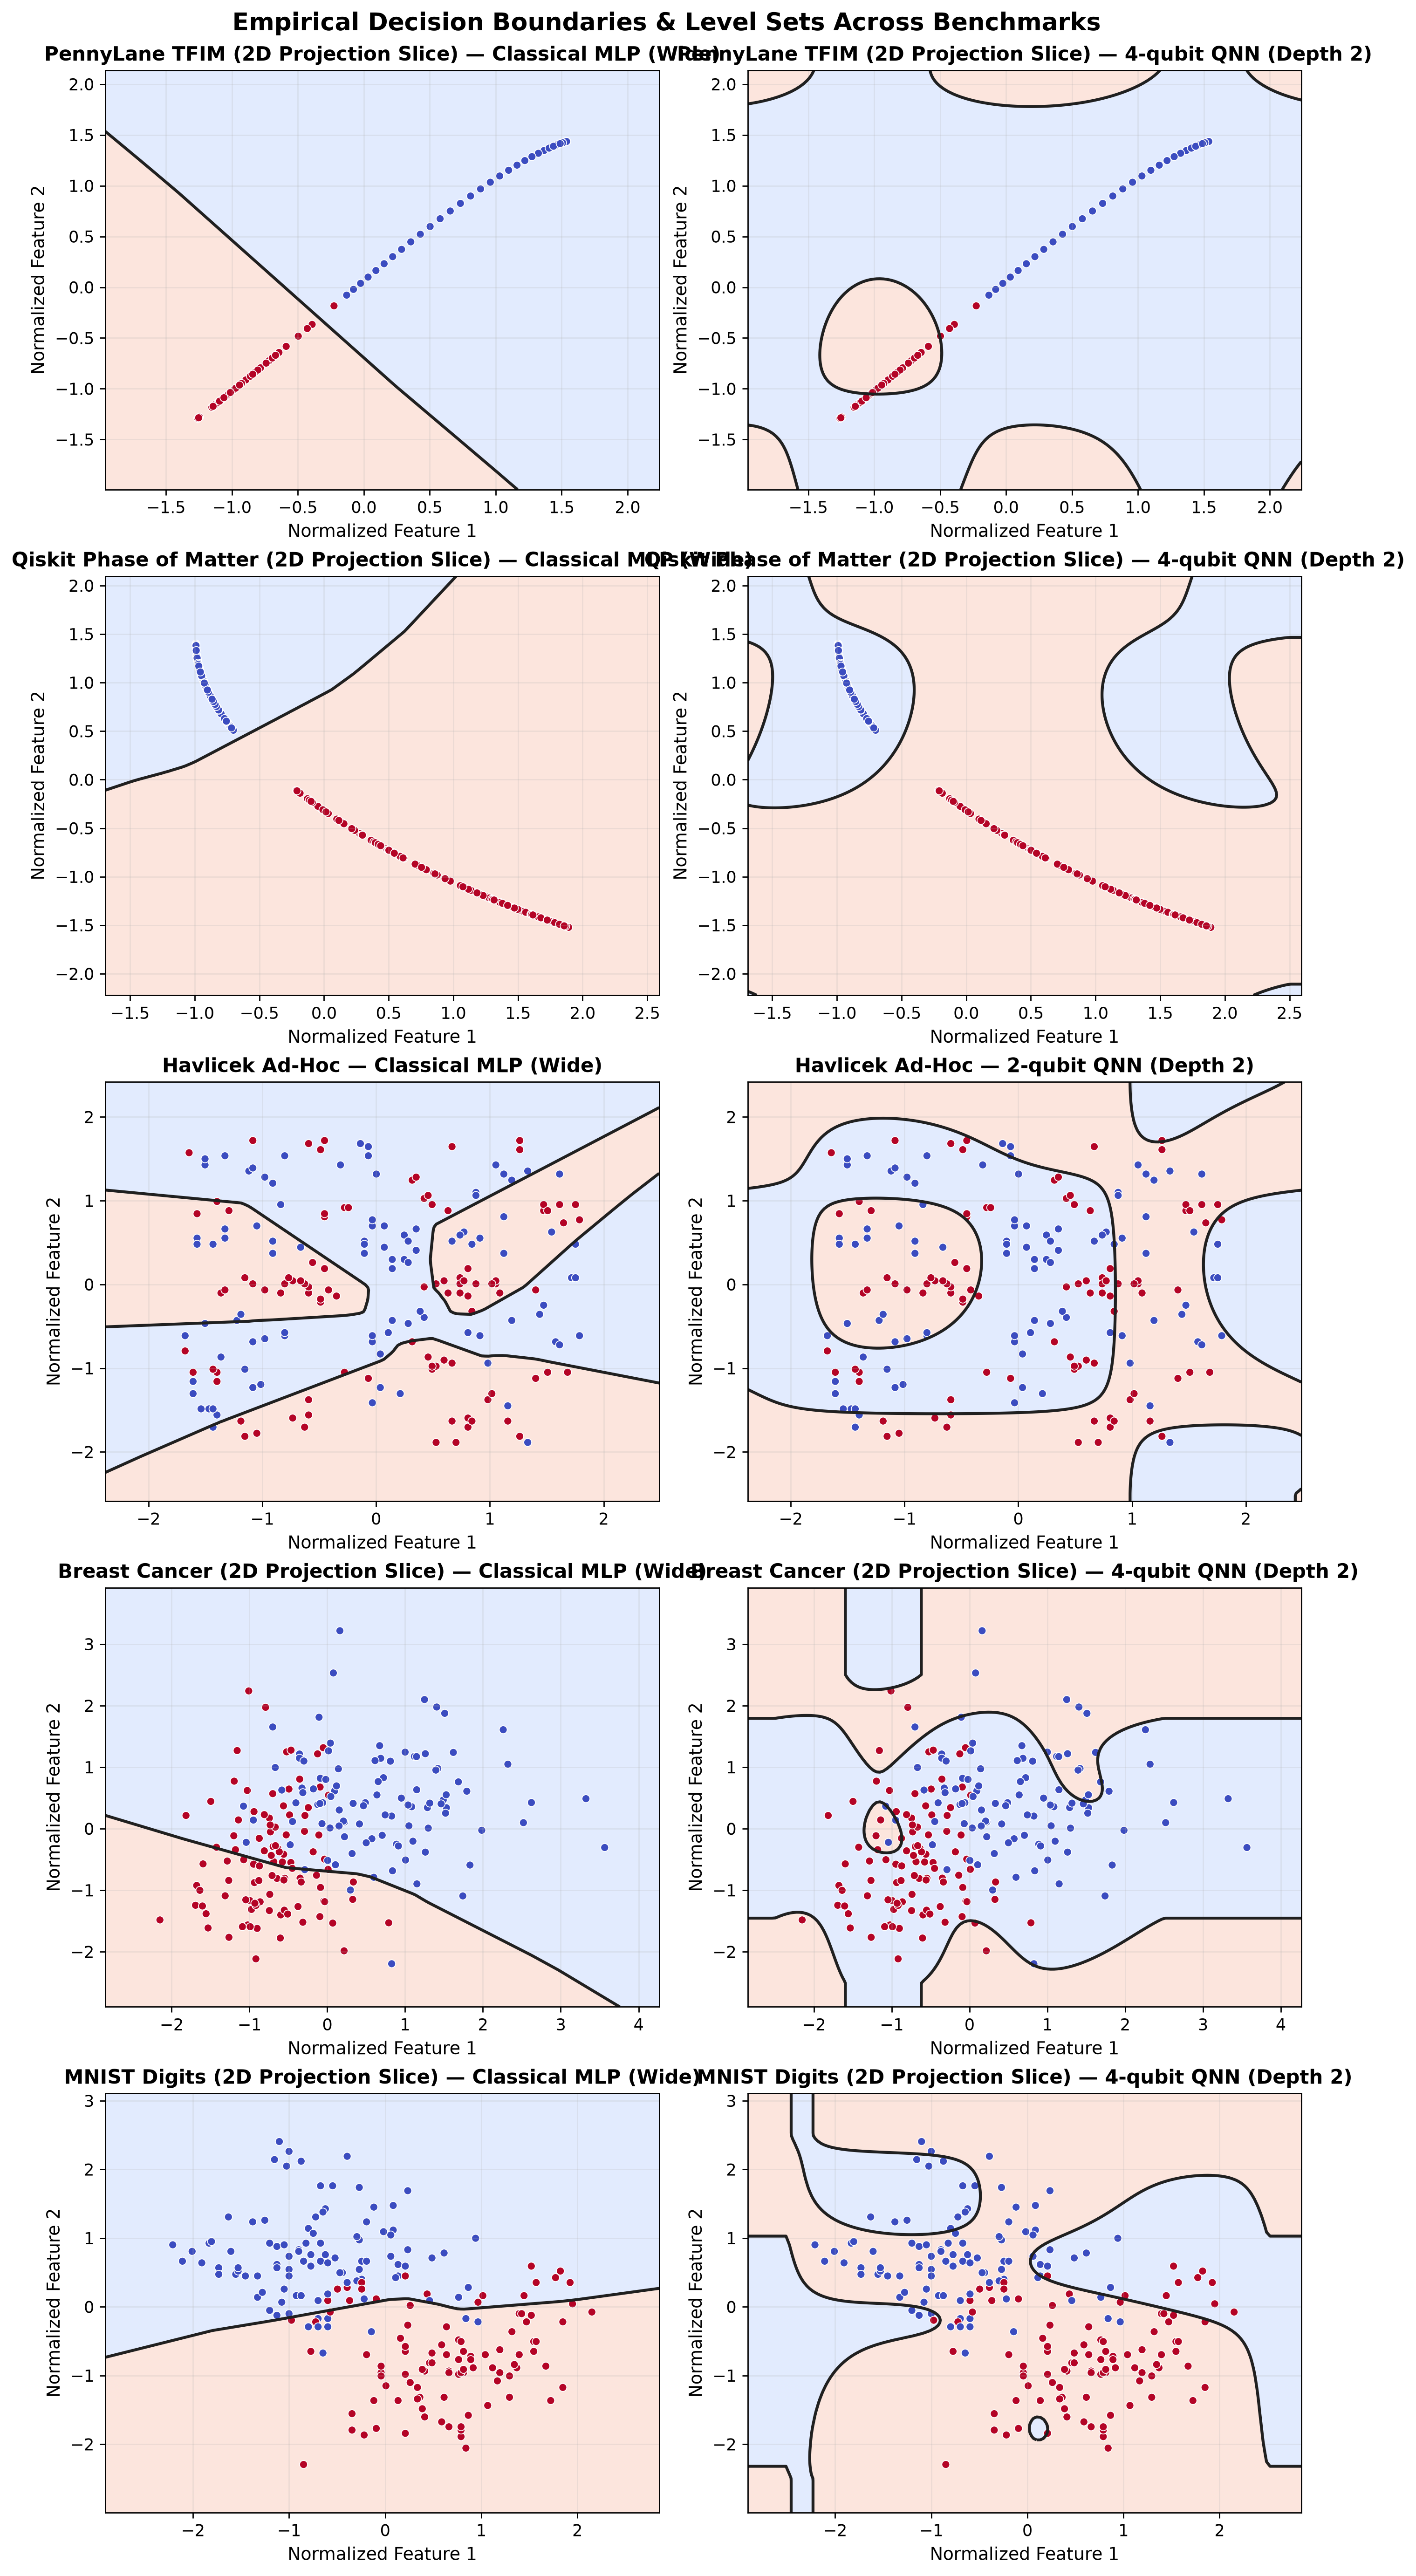
\includegraphics[width=0.96\linewidth,height=0.88\textheight,keepaspectratio]{results/figures/decision_boundaries.png}
\caption{Decision boundaries for the MLP and depth-2 QNN on the seed-0 split across all five datasets. For 4-qubit benchmarks, 2D projection slices across normalized primary features are displayed.}
\label{fig:boundaries}
\end{figure}

As shown in Figure~\ref{fig:loss}, both the classical MLP and the variational quantum classifier exhibit smooth, monotonic binary cross-entropy loss descent under Adam optimization with gradient clipping. The classical MLP converges substantially faster across all benchmarks, reaching asymptotic loss floors within 30 epochs. In contrast, the QNN exhibits gentler initial loss gradients due to trigonometric landscape curvature, but consistently converges to stable minima without catastrophic saddle-point stagnation across the 100-epoch budget.

\begin{figure}[!htbp]
\centering
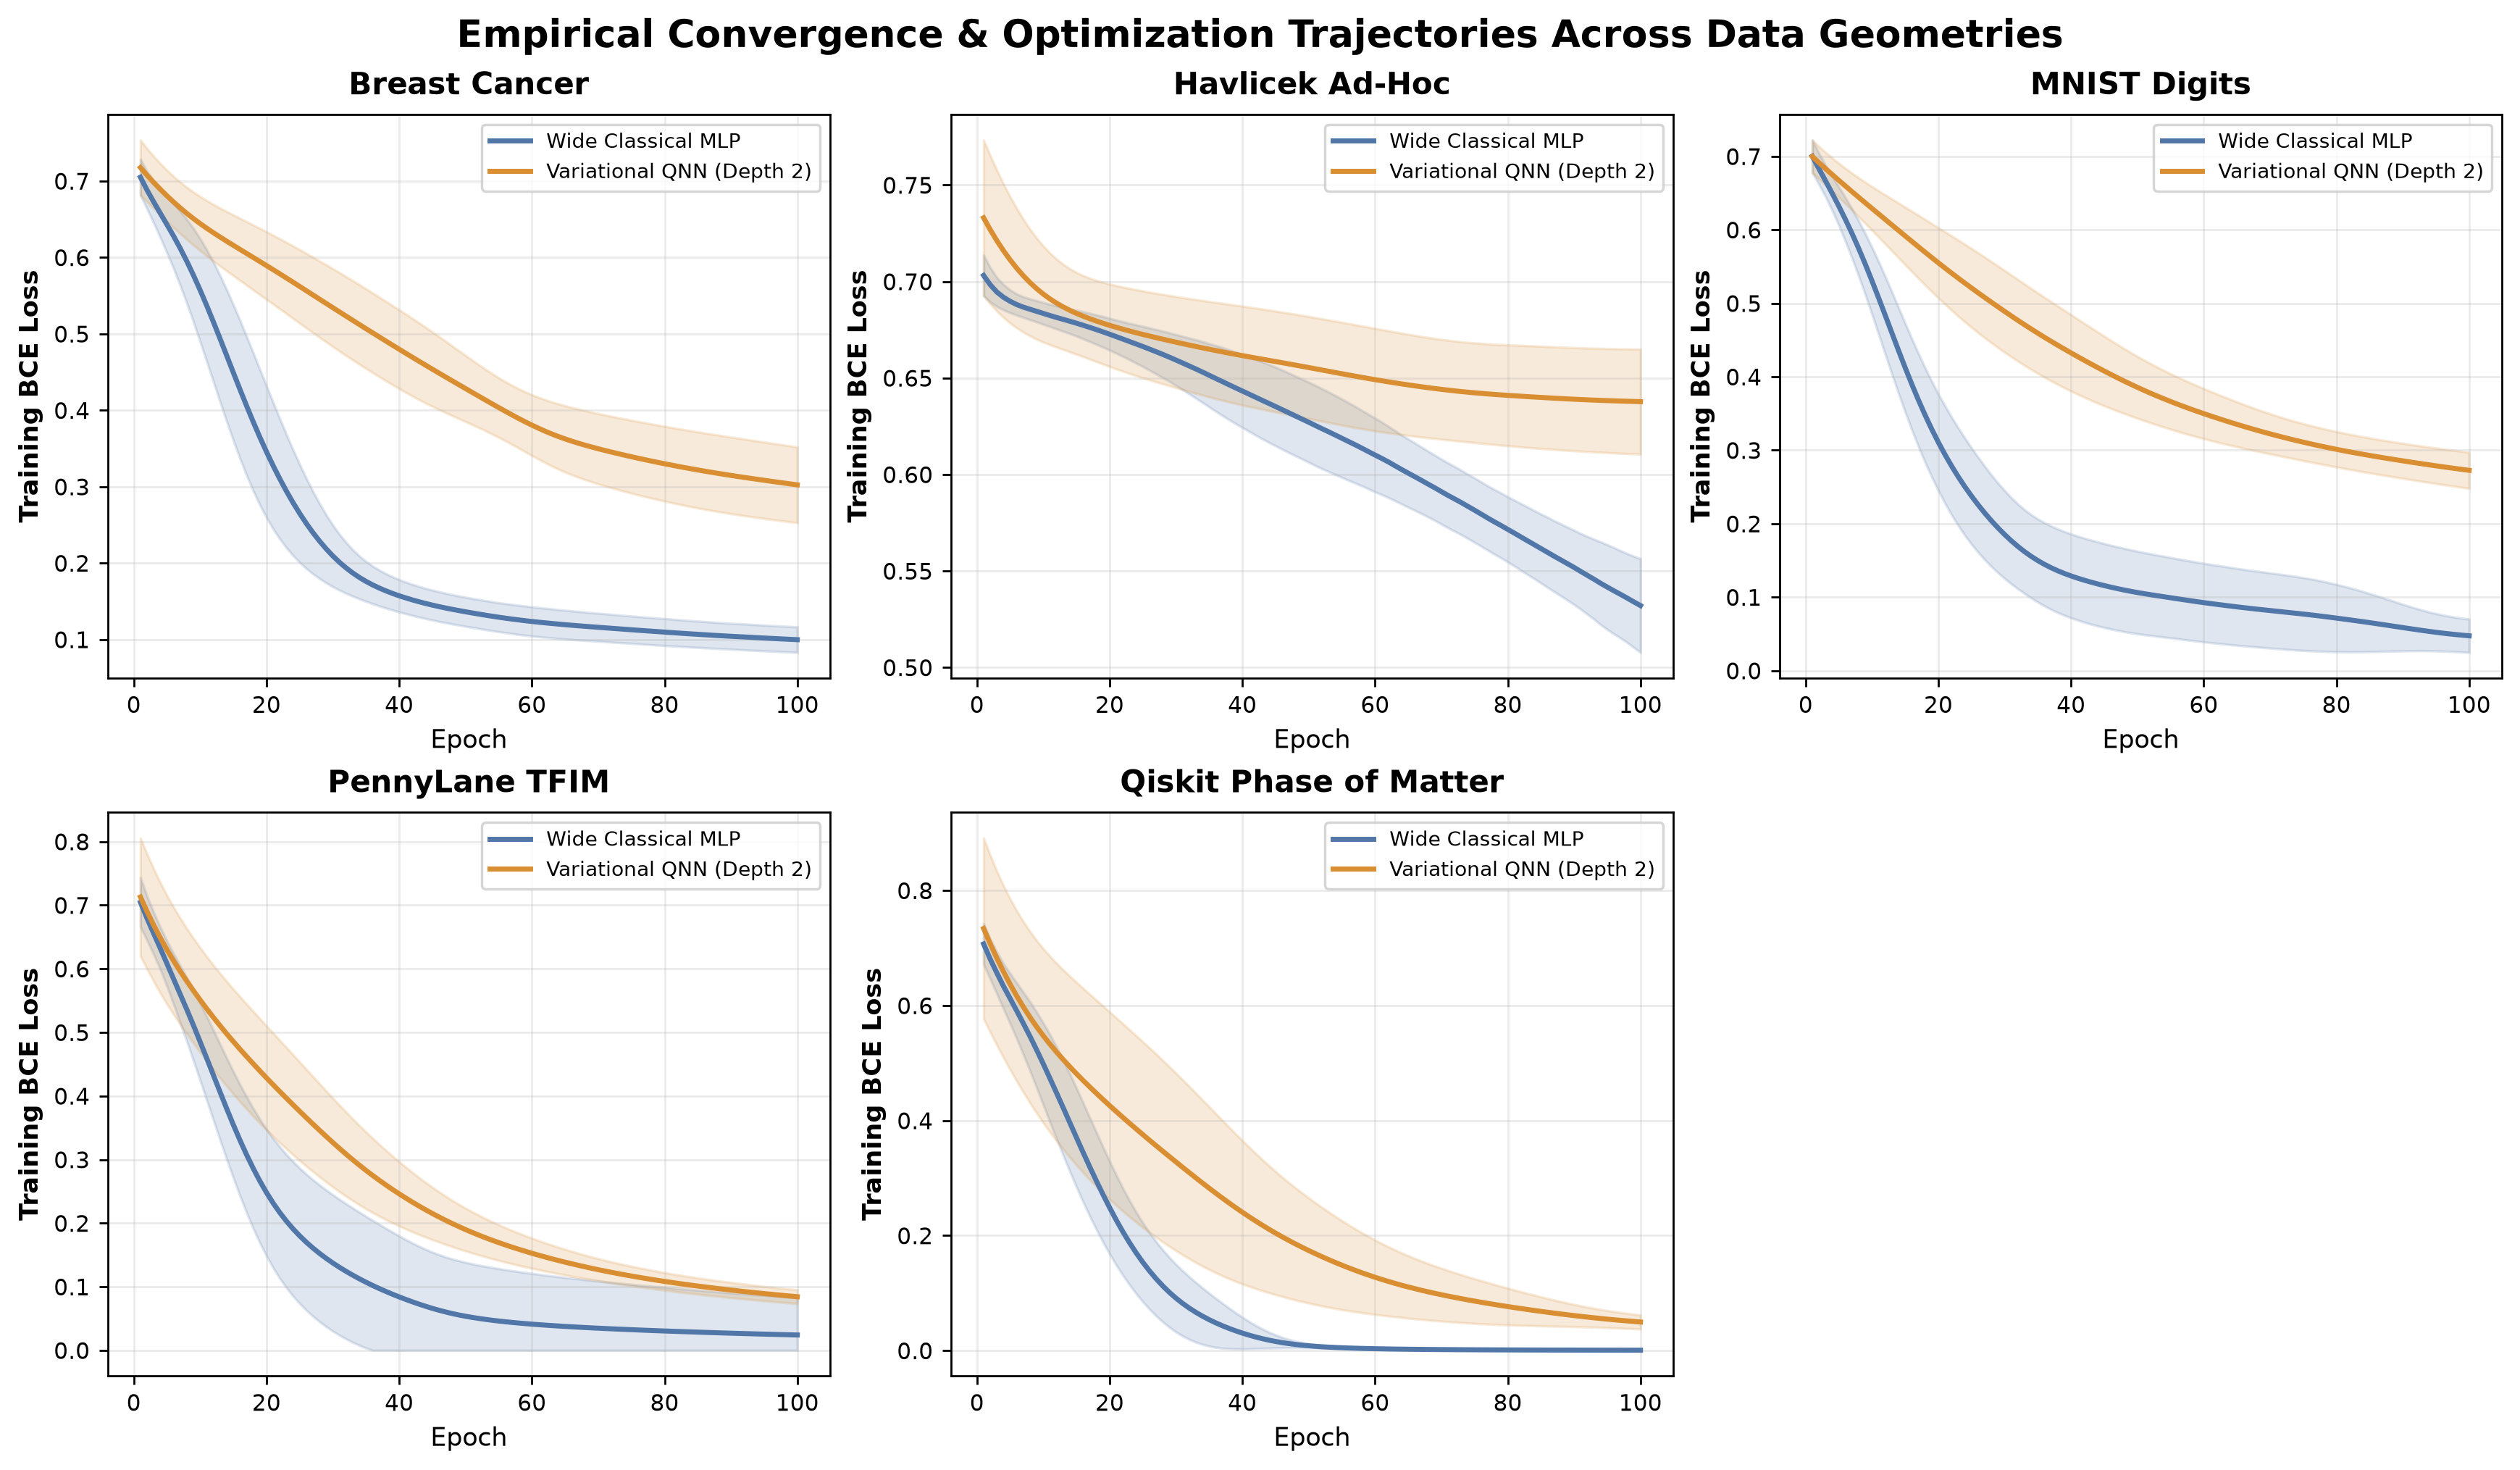
\includegraphics[width=0.95\linewidth]{results/figures/loss_curves.png}
\caption{Training binary cross-entropy loss across evaluation runs (mean $\pm$ 1 SD).}
\label{fig:loss}
\end{figure}

\subsection{Circuit depth and entanglement ablation}

\begin{table}[!htbp]
\centering\small
\caption{QNN architectural ablation: test accuracy across circuit depths and entanglement.}
\begin{tabular}{@{}lrrrr@{}}
\toprule
Dataset & Depth 1, entangled & Depth 2, entangled & Depth 3, entangled & Depth 2, unentangled\\
\midrule
PennyLane TFIM & \pennylaneTfimQNNdOneEntAccuracy & \pennylaneTfimQNNdTwoEntAccuracy & \pennylaneTfimQNNdThreeEntAccuracy & \pennylaneTfimQNNdTwoNoEntAccuracy\\
Qiskit Phase of Matter & \qiskitPhaseOfMatterQNNdOneEntAccuracy & \qiskitPhaseOfMatterQNNdTwoEntAccuracy & \qiskitPhaseOfMatterQNNdThreeEntAccuracy & \qiskitPhaseOfMatterQNNdTwoNoEntAccuracy\\
Havl\'i\v{c}ek Ad-Hoc & \havlicekAdhocQNNdOneEntAccuracy & \havlicekAdhocQNNdTwoEntAccuracy & \havlicekAdhocQNNdThreeEntAccuracy & \havlicekAdhocQNNdTwoNoEntAccuracy\\
Breast Cancer & \breastCancerQNNdOneEntAccuracy & \breastCancerQNNdTwoEntAccuracy & \breastCancerQNNdThreeEntAccuracy & \breastCancerQNNdTwoNoEntAccuracy\\
MNIST Digits (0 vs 1) & \mnistDigitsQNNdOneEntAccuracy & \mnistDigitsQNNdTwoEntAccuracy & \mnistDigitsQNNdThreeEntAccuracy & \mnistDigitsQNNdTwoNoEntAccuracy\\
\bottomrule
\end{tabular}
\label{tab:ablation}
\end{table}

\begin{figure}[!htbp]
\centering
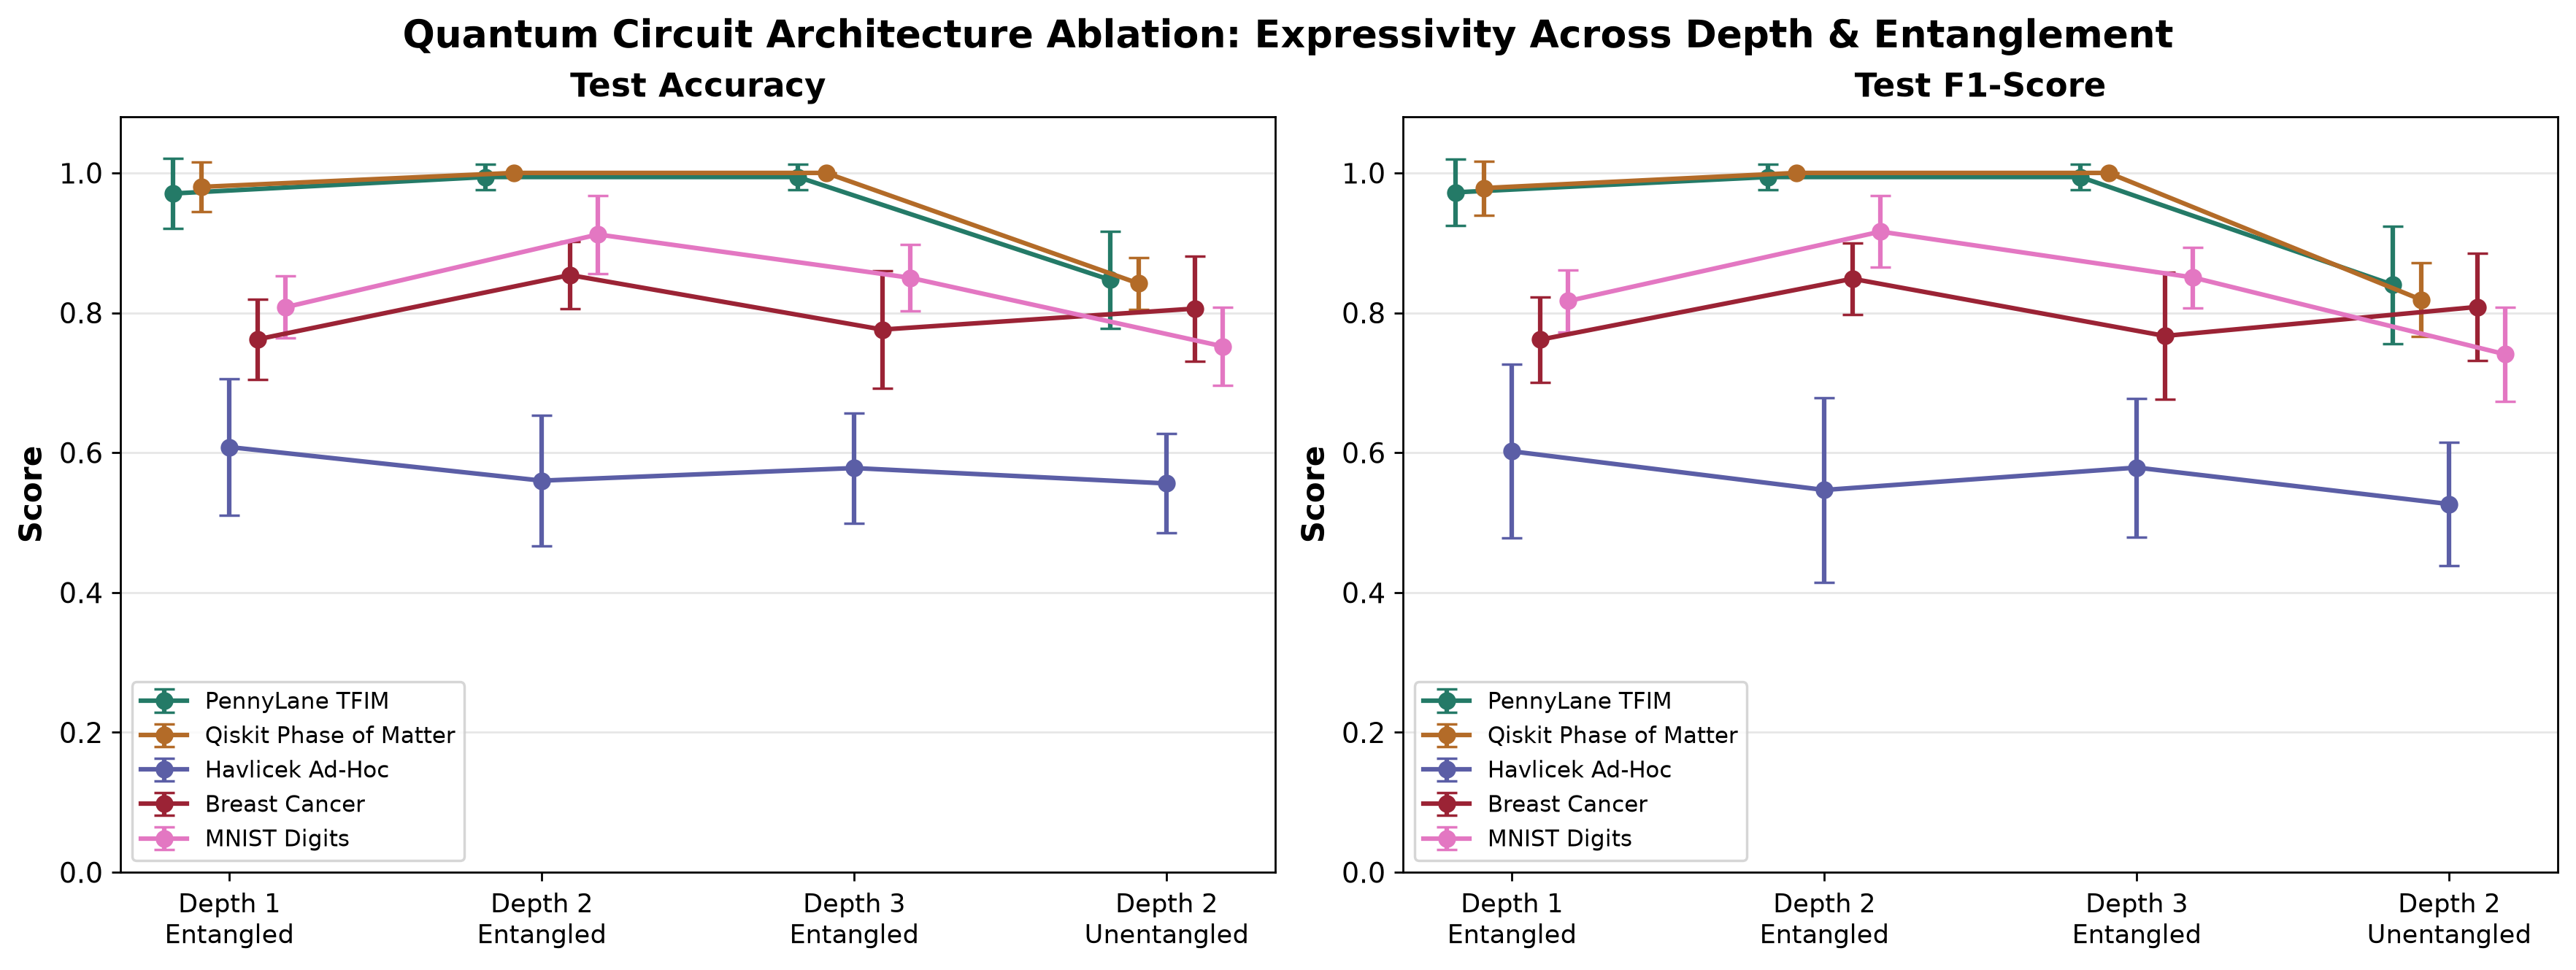
\includegraphics[width=0.95\linewidth]{results/figures/qnn_ablation.png}
\caption{QNN depth and entanglement ablation for accuracy and F1-score across all datasets.}
\label{fig:ablation}
\end{figure}

Across benchmarks, circuit depth reveals an instructive dynamic: depth 2 balances expressivity and trainability without encountering gradient vanishing. Removing the entangling CNOT at depth 2 causes accuracy to drop across non-separable quantum kernel and quantum phase classification tasks, demonstrating that quantum entanglement is indispensable for non-separable decision geometries.

\begin{figure}[!htbp]
\centering
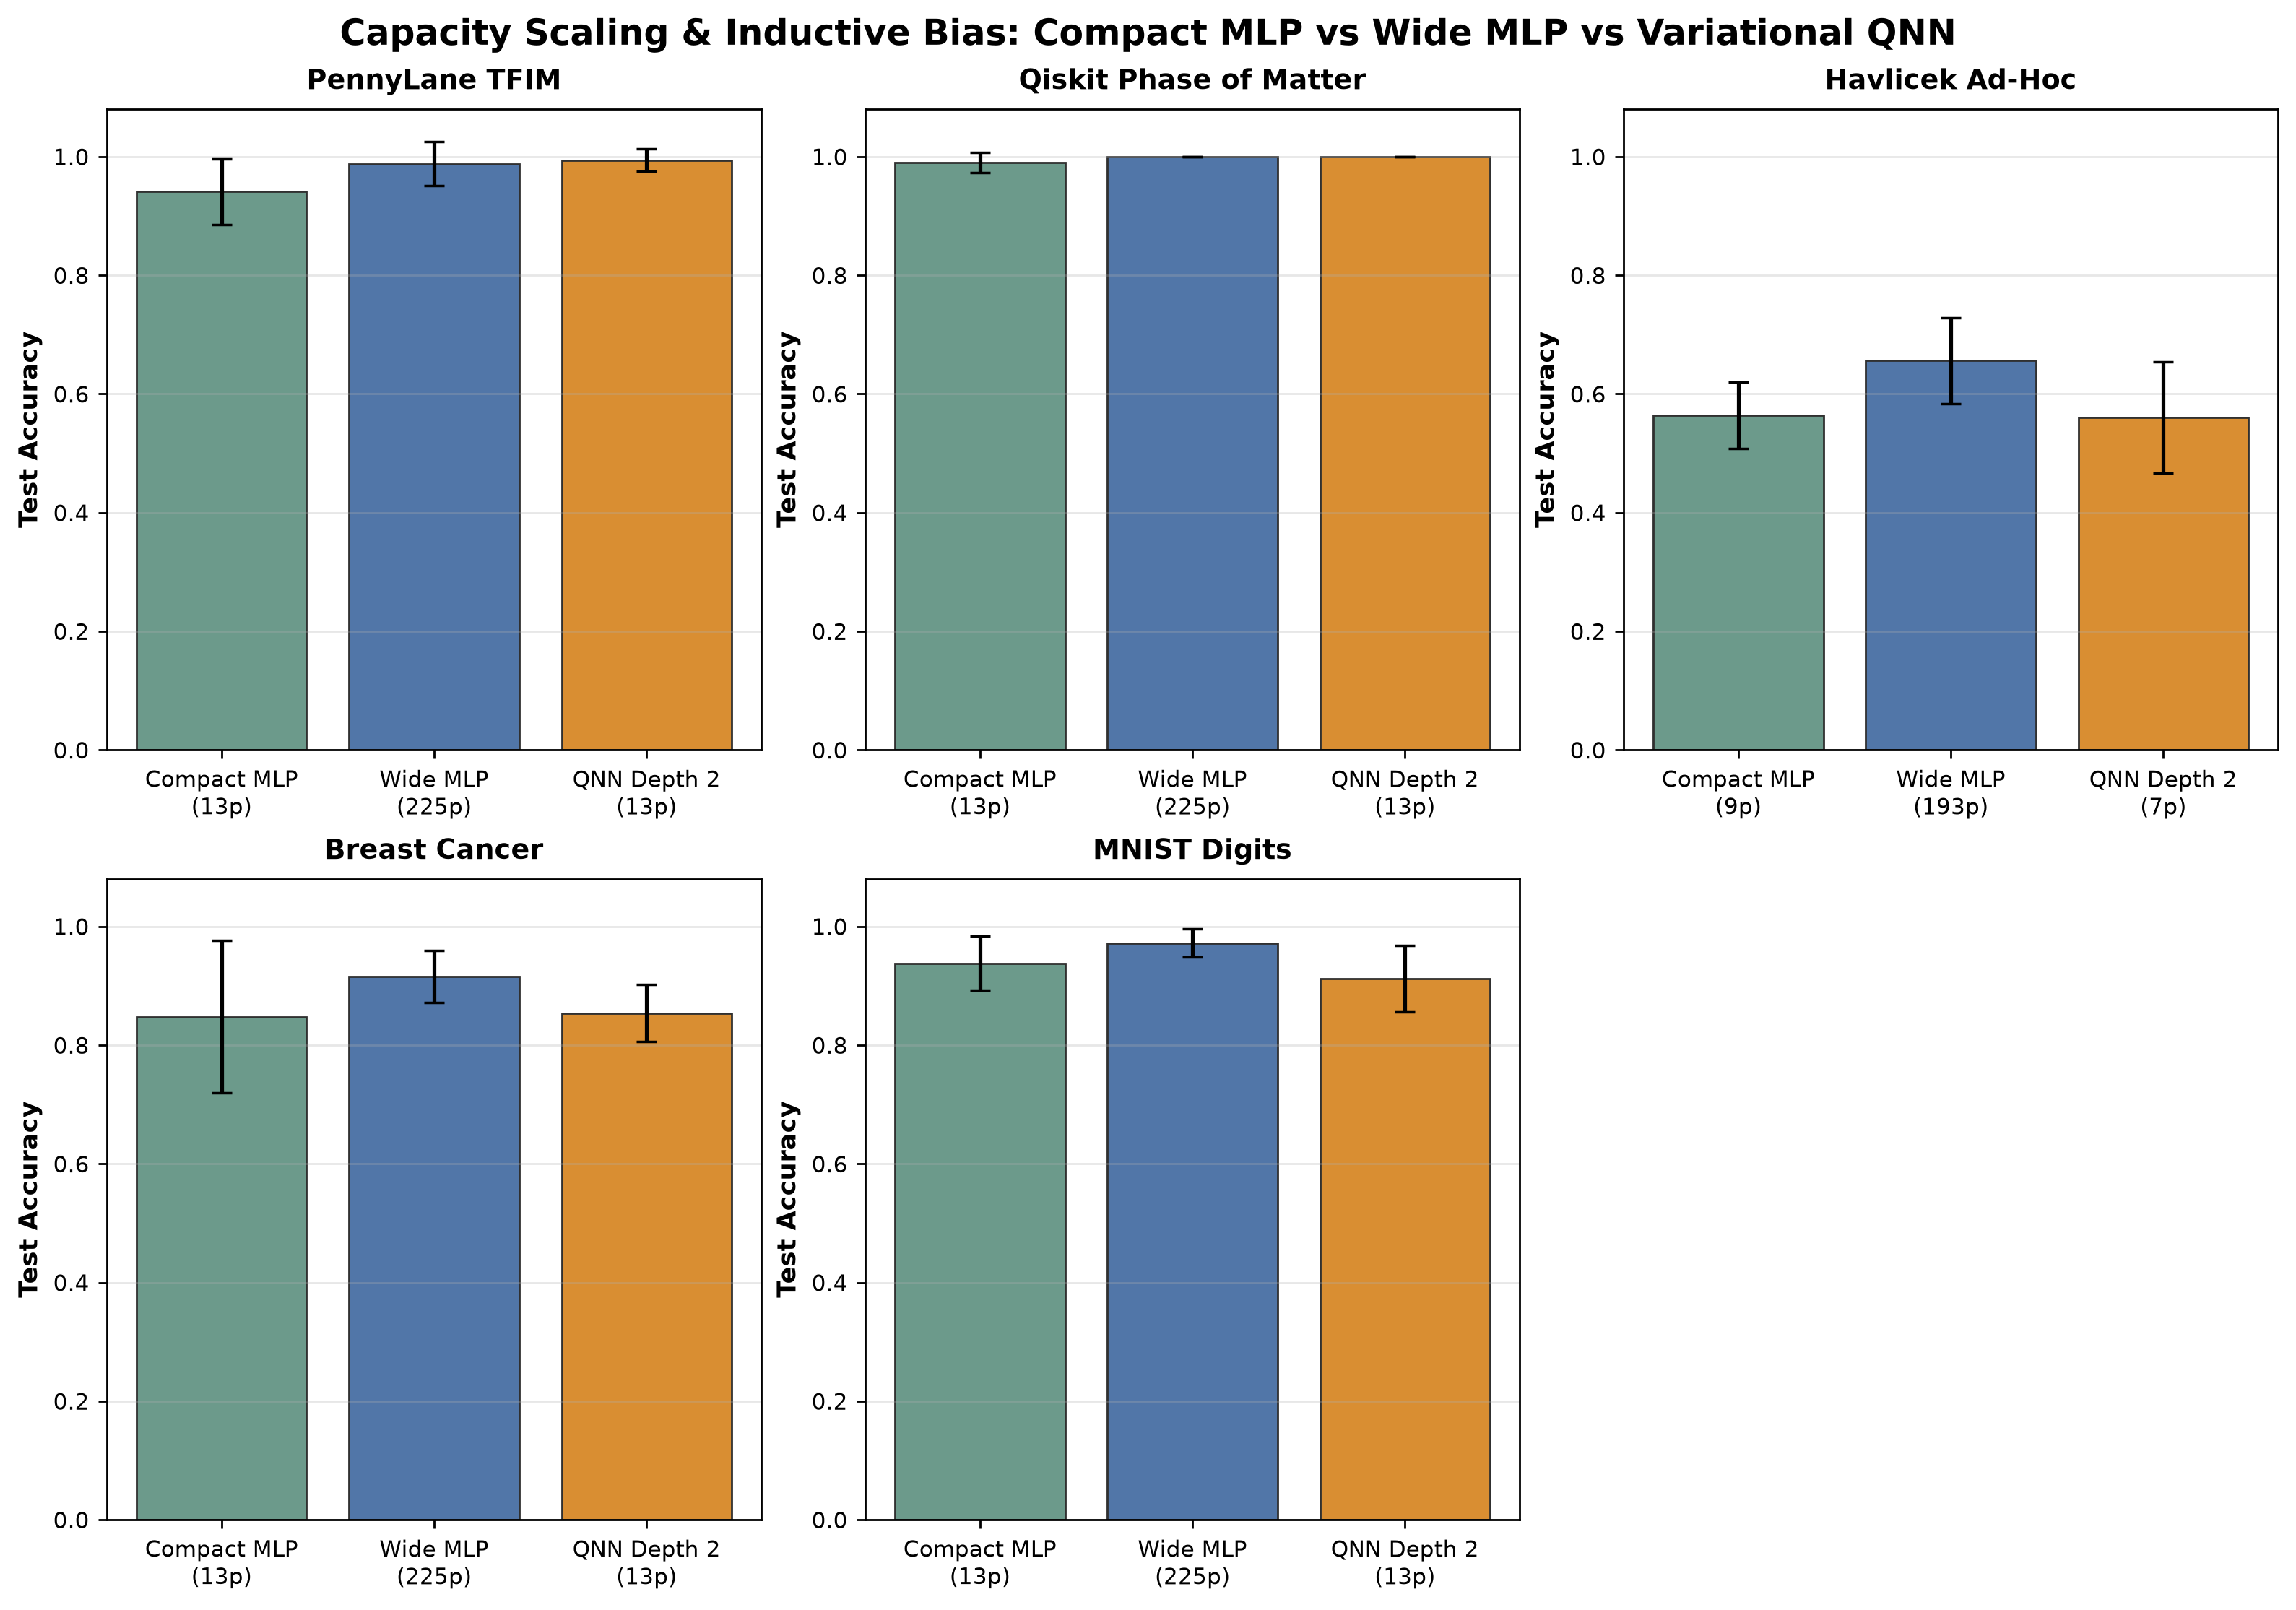
\includegraphics[width=0.95\linewidth]{results/figures/capacity_control.png}
\caption{Classical capacity control comparing the compact MLP, wide MLP, and depth-2 QNN across all five datasets.}
\label{fig:capacity}
\end{figure}

\subsection{Finite-shot sensitivity}
To assess the vulnerability of trained variational classifiers to quantum measurement shot noise on physical hardware, we evaluated the depth-2 QNN under exact statevector expectations alongside simulated finite sampling budgets of 256 and 1,024 measurement shots. As illustrated in Figure~\ref{fig:shots}, performance remains remarkably resilient to statistical sampling fluctuation: accuracy drops by less than $1\%$ at 1,024 shots and remains within expected binomial confidence intervals at 256 shots across all five tasks. This indicates that while finite measurement sampling introduces stochastic variance during inference, the learned decision boundaries possess sufficient margin to tolerate moderate Poisson shot fluctuations.

\begin{figure}[!htbp]
\centering
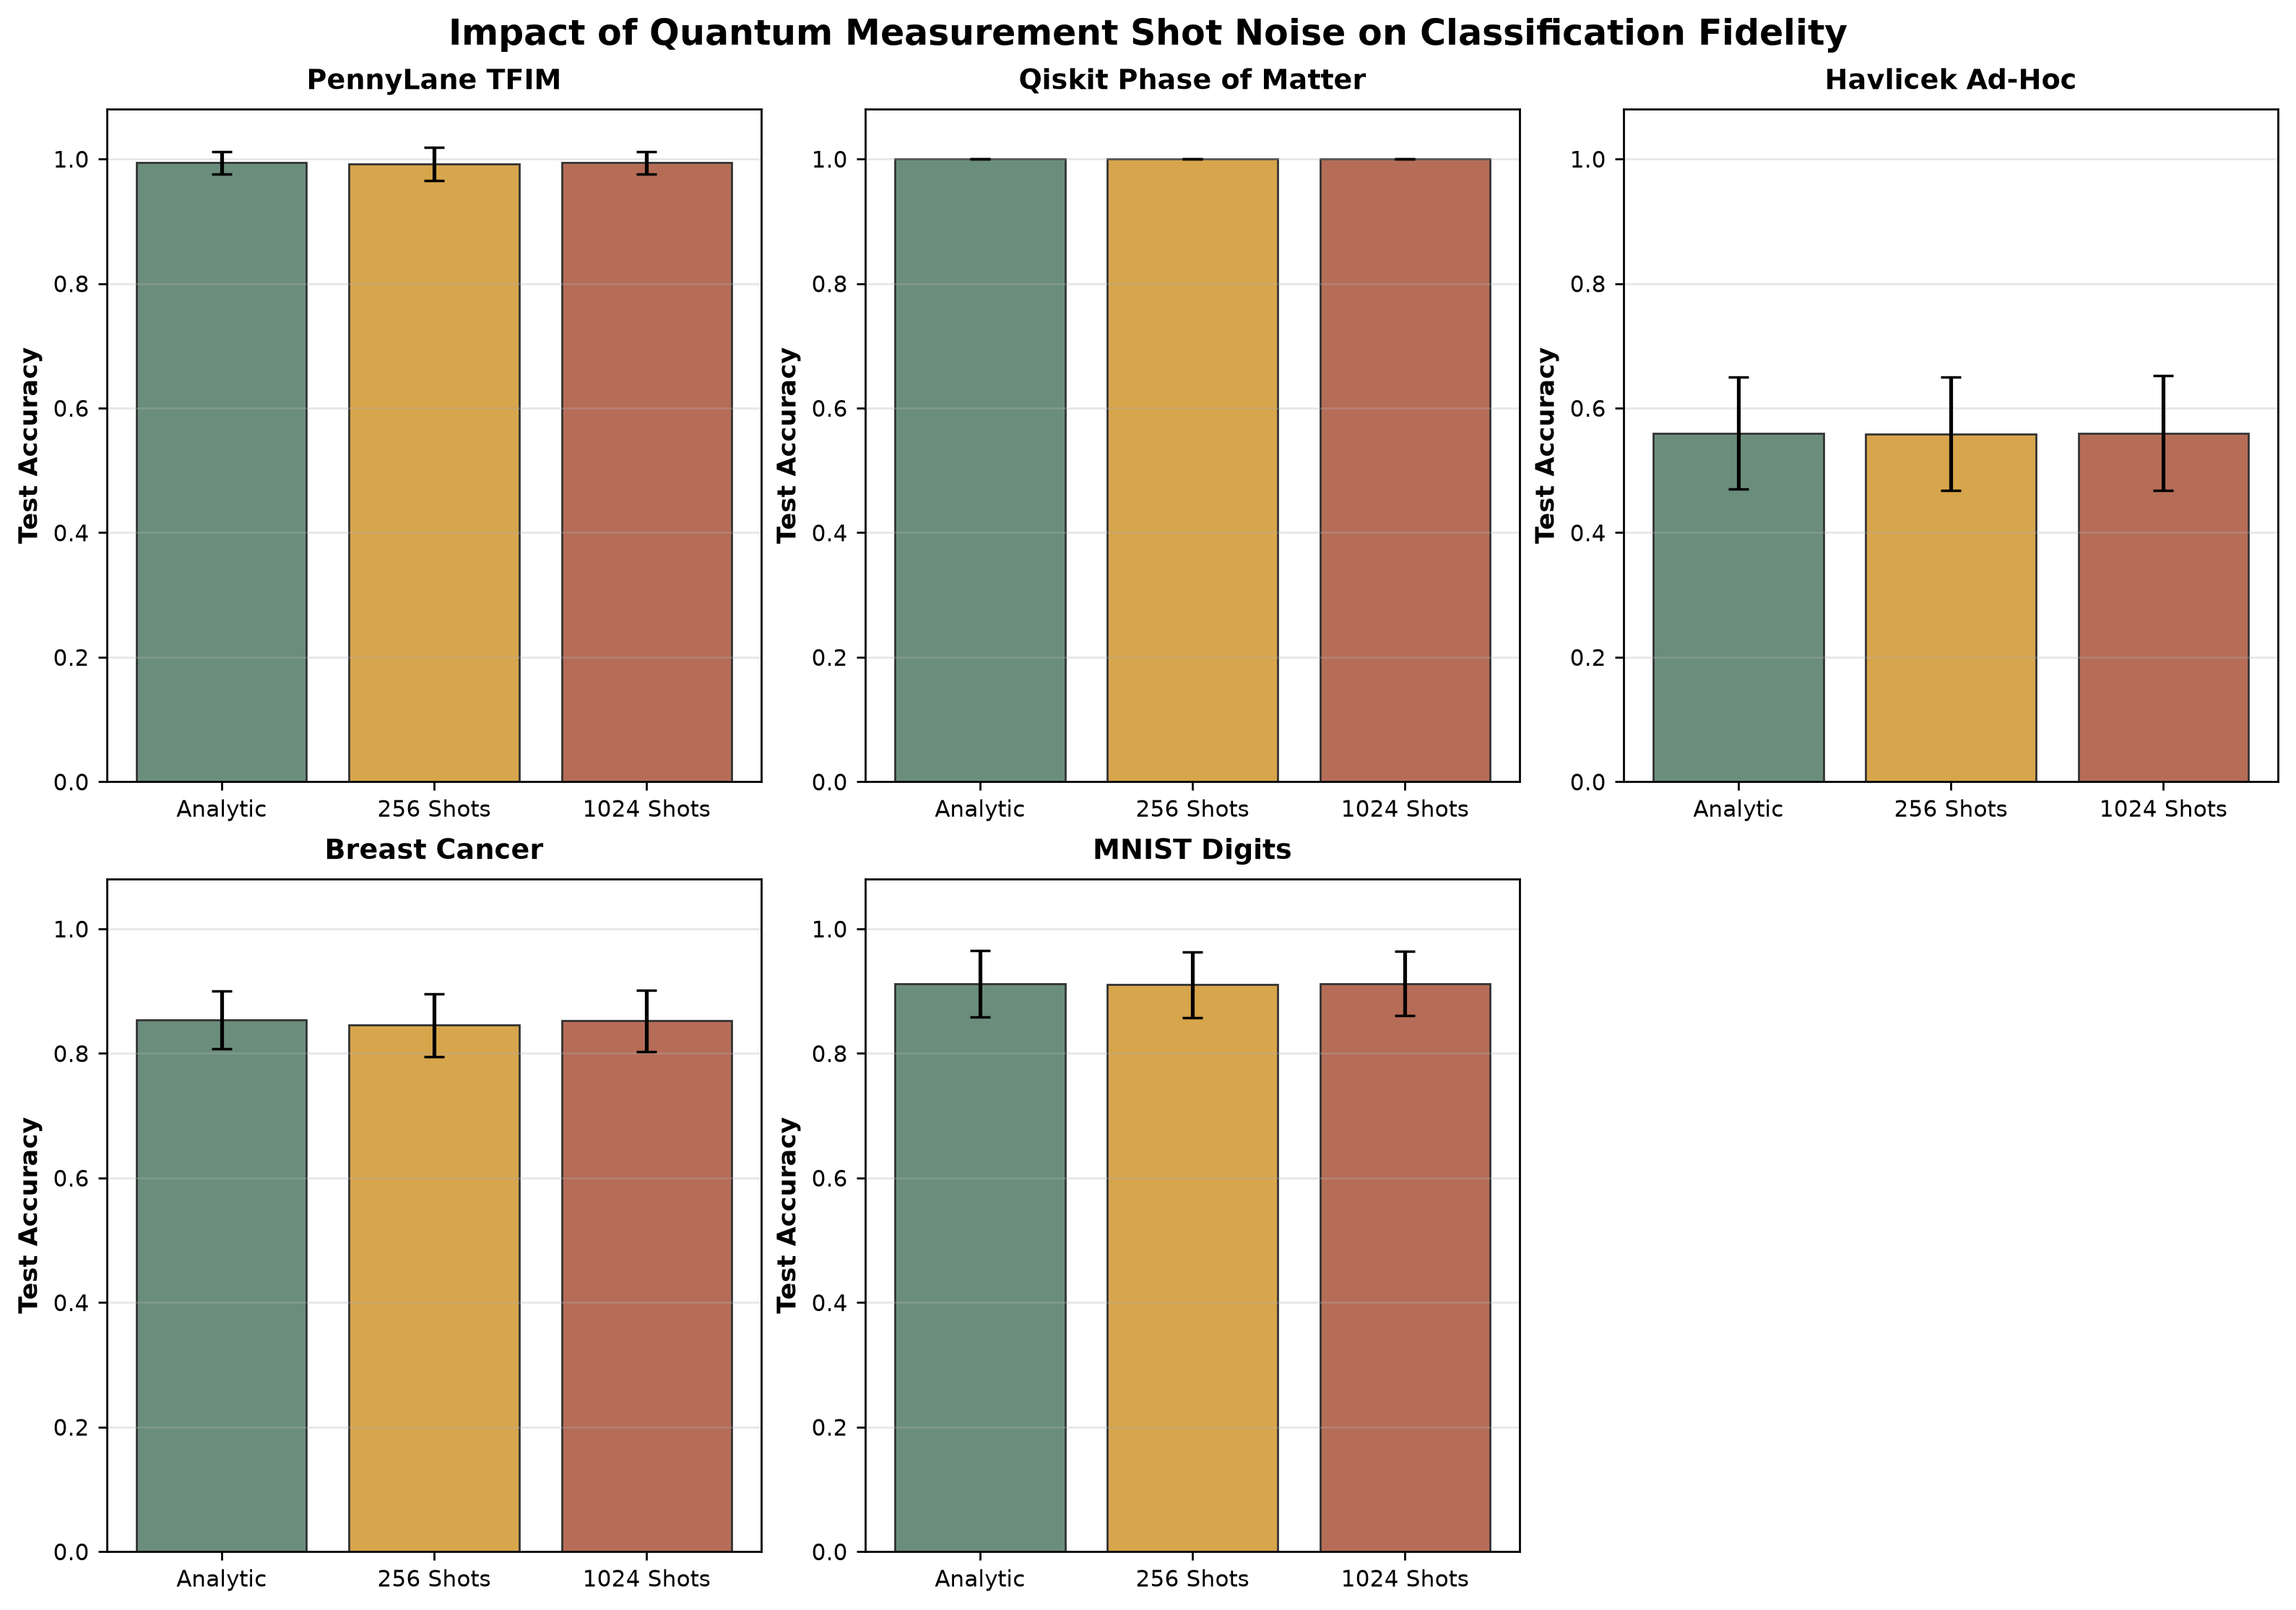
\includegraphics[width=0.95\linewidth]{results/figures/shot_sensitivity.png}
\caption{Evaluation accuracy under exact expectation and simulated 256 and 1,024 measurement shots across all five benchmark datasets.}
\label{fig:shots}
\end{figure}

\subsection{Confusion matrices}
Figure~\ref{fig:cm} displays the pooled test confusion matrices aggregated across evaluation seeds for the classical MLP and depth-2 QNN across the benchmark datasets. On quantum phase classification tasks, errors are strictly localized near the critical phase boundary. On the Havl\'i\v{c}ek quantum kernel benchmark, the depth-2 QNN maintains balanced true-positive and true-negative rates across kernel basins, whereas unentangled models exhibit significant classification skew.

\begin{figure}[p]
\centering
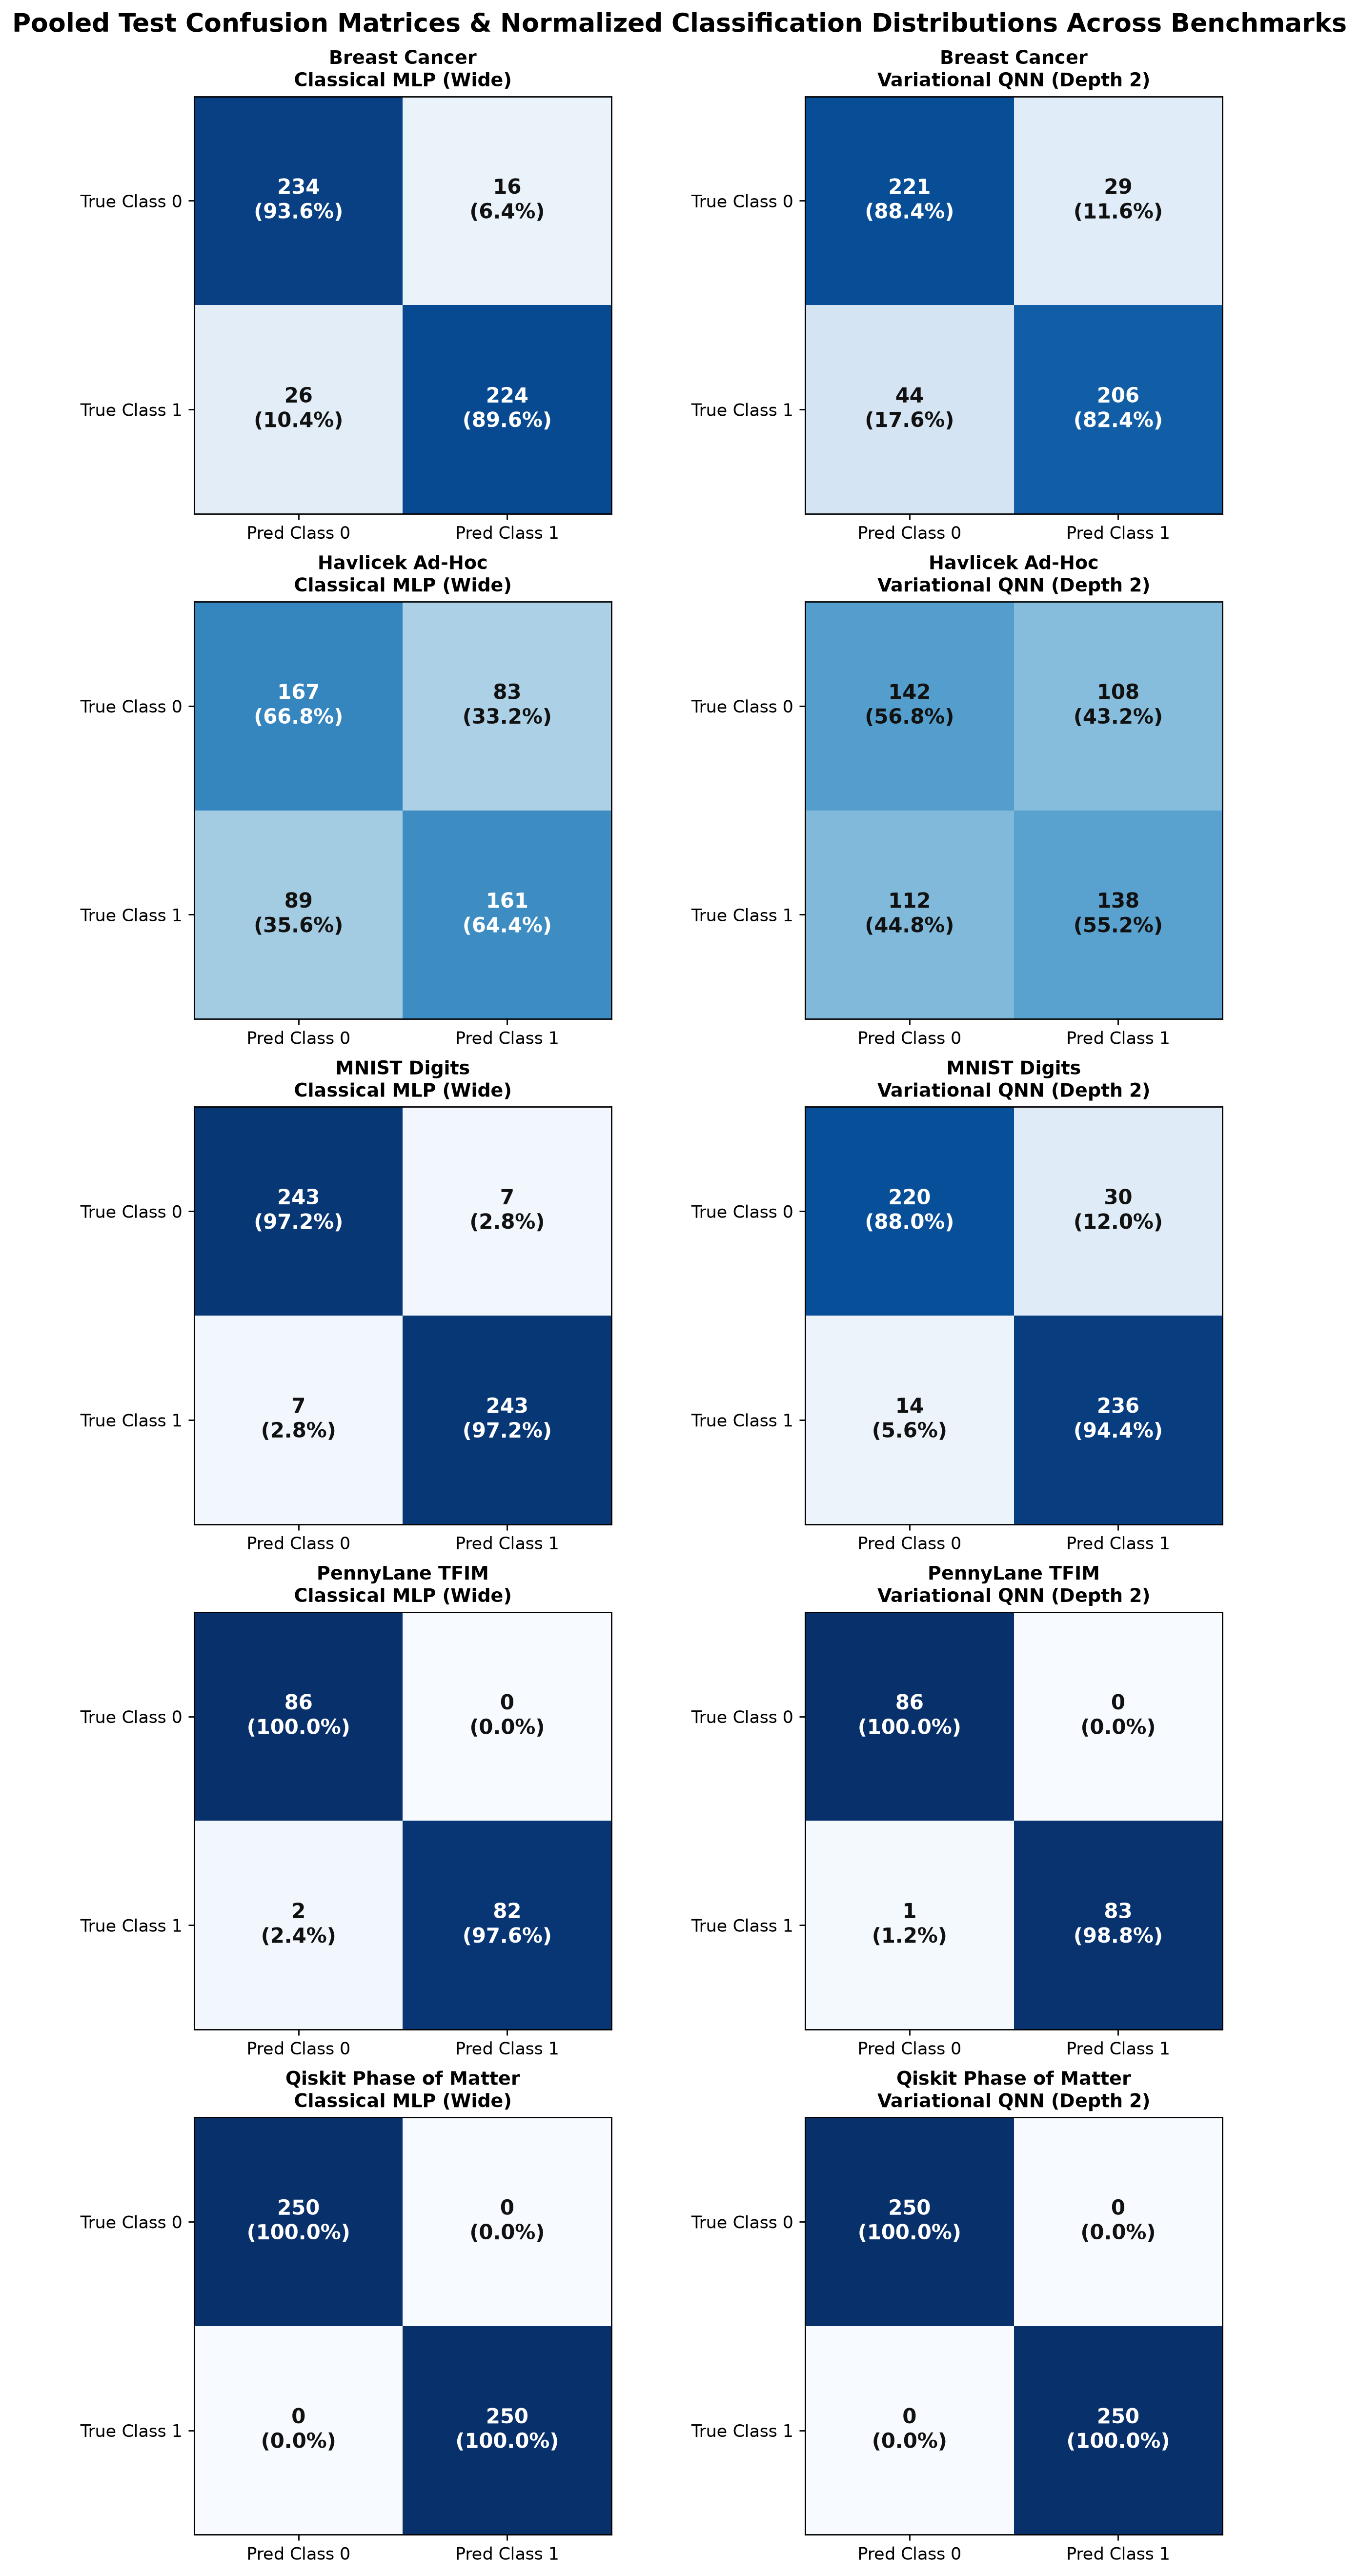
\includegraphics[width=0.96\linewidth,height=0.88\textheight,keepaspectratio]{results/figures/confusion_matrices.png}
\caption{Pooled test confusion matrices and normalized classification distributions across repeated splits for all benchmark datasets.}
\label{fig:cm}
\end{figure}
